\section{原子的精细结构: 电子的自旋}
\subsection{史特恩(Stern)-盖拉赫(Gerlach)实验}
\begin{figure}[!htb]
\centering
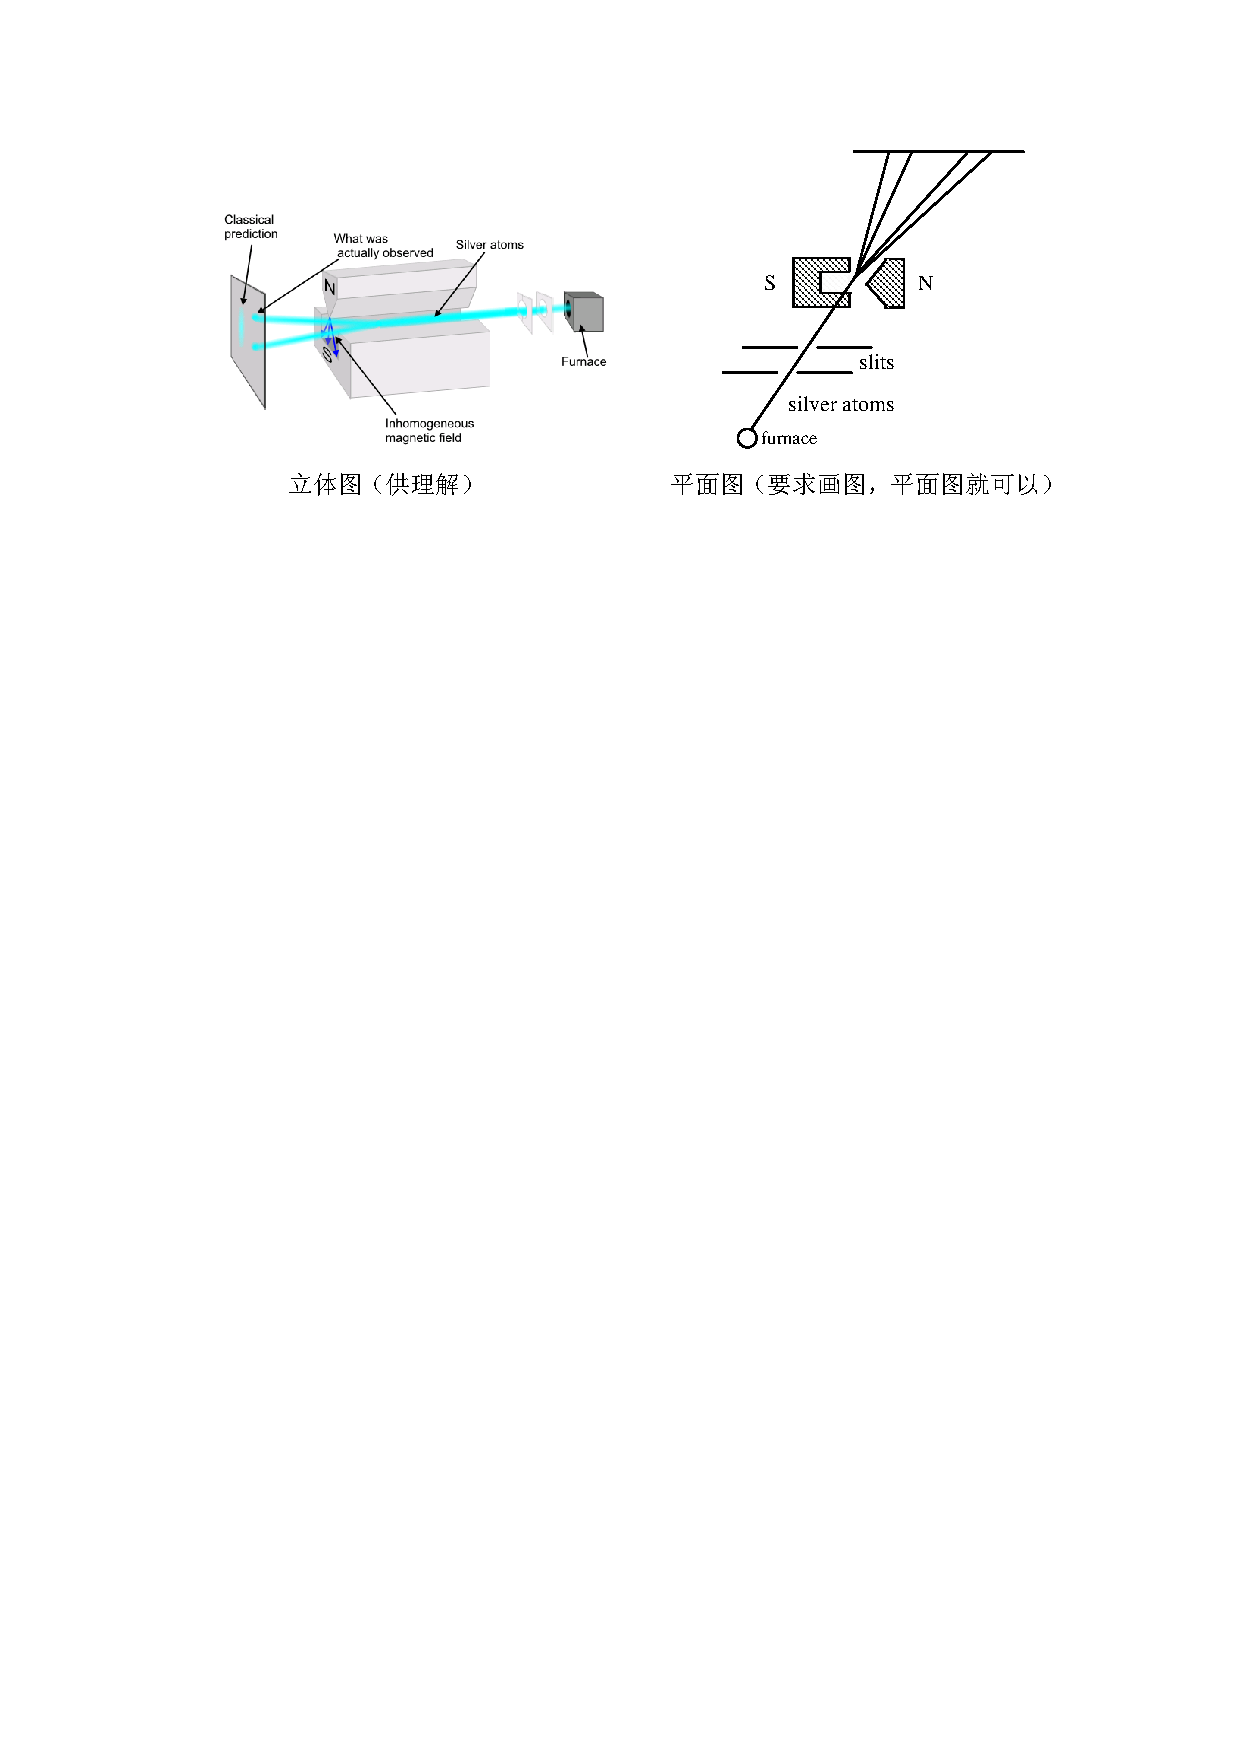
\includegraphics[width=0.8\textwidth]{fig05.pdf}
\caption{\label{fig05}特恩-盖拉赫实验}
\end{figure}
原子射线束通过一个不均匀的磁场区域, 射线束在磁场作用下发生偏折, 最后落在屏上. 如果原子磁矩的方向是可以任意取向的, 则屏上形成一片黑斑. 而实验发现屏上形成了几条清晰的黑斑, 表明银原子的\textbf{磁矩}($\mu$)只能取几个特定的方向, 从而验证了原子角动量的投影是量子化的.  在磁场中, 原子受力$f\varpropto\frac{\textrm{d}B}{\textrm{d}z}\mu$. \textbf{结果}如图\ref{fig06}.
\begin{figure}[!htb]
\centering
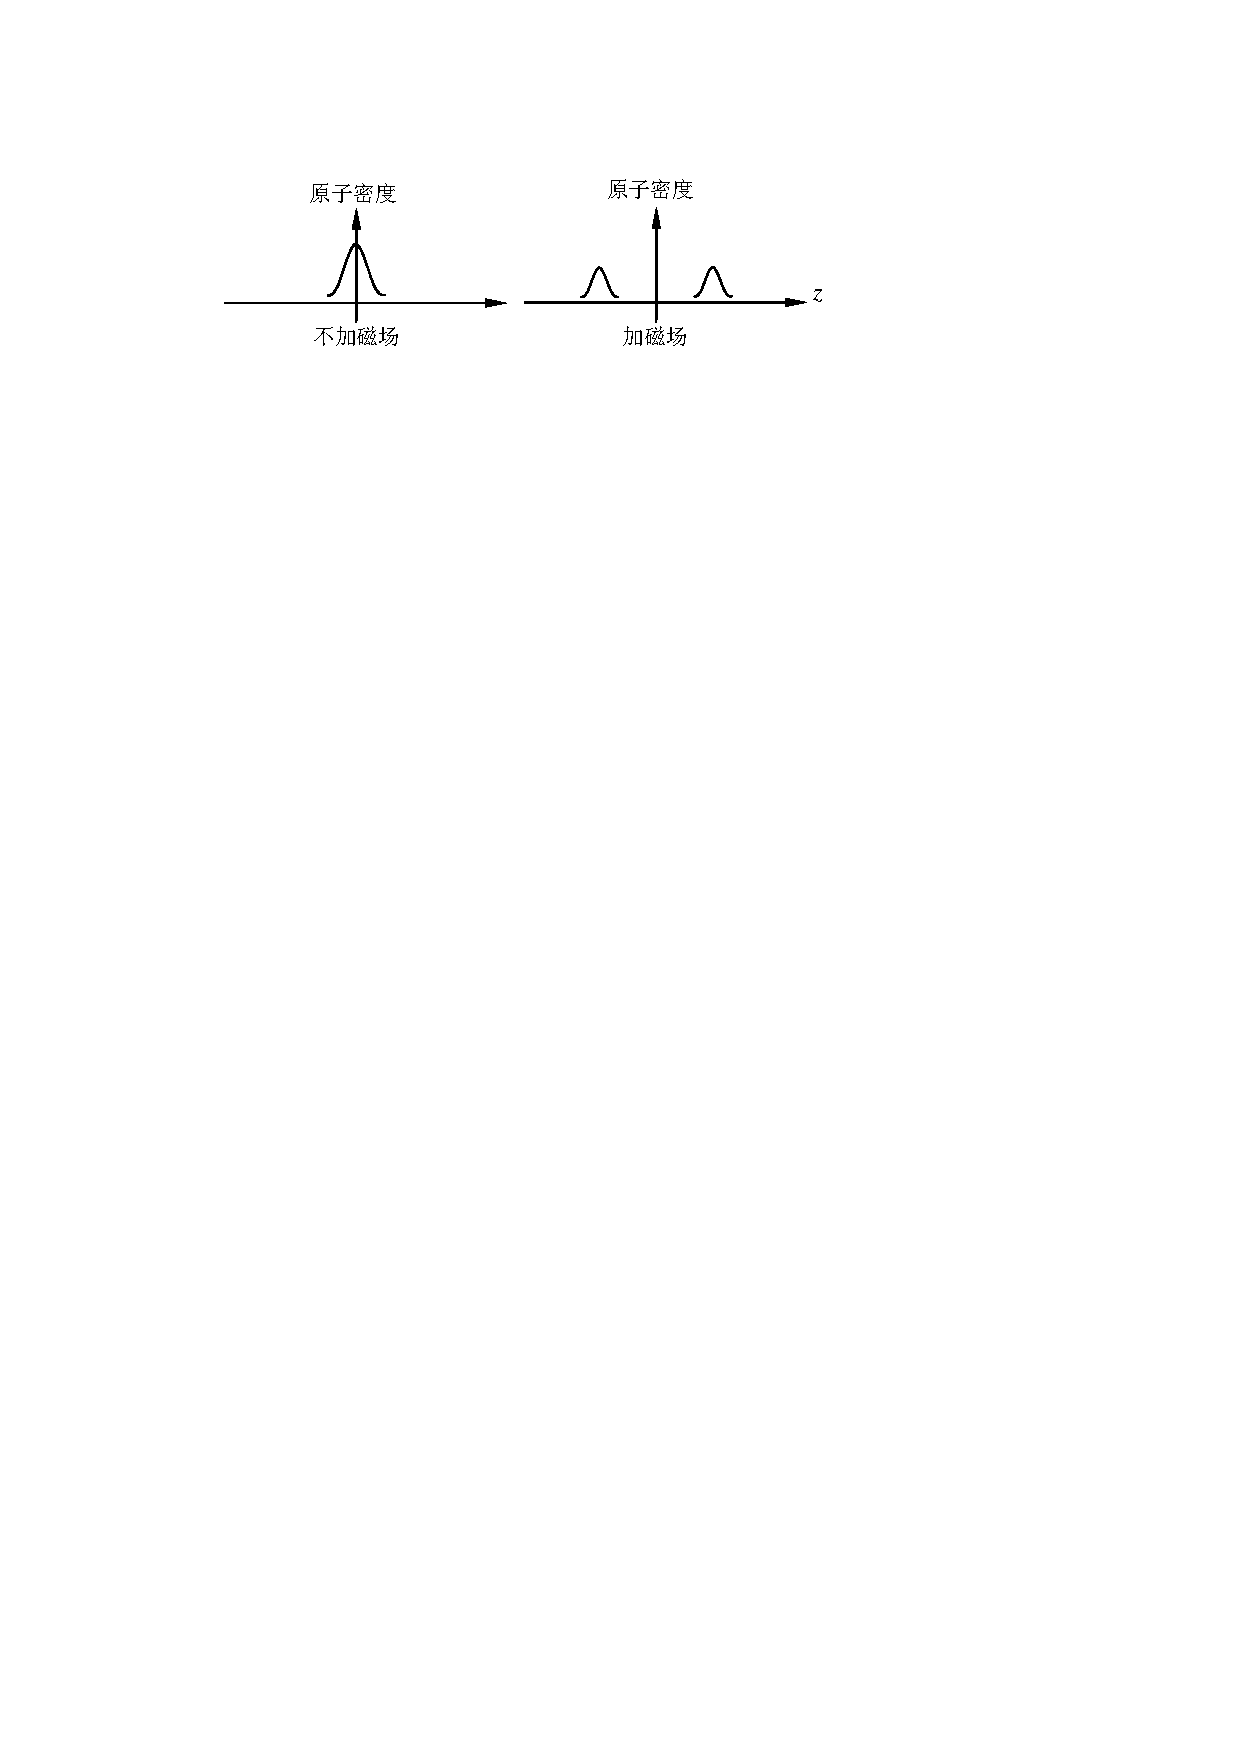
\includegraphics[width=0.6\textwidth]{fig06.pdf}
\caption{\label{fig06}史特恩-盖拉赫实验结果}
\end{figure}


\subsection{塞曼(Zeeman)效应}
塞曼效应是原子的光谱线在外磁场中出现分裂的现象. 
\begin{figure}[!htb]
\begin{minipage}[b]{0.48\textwidth}
\centering
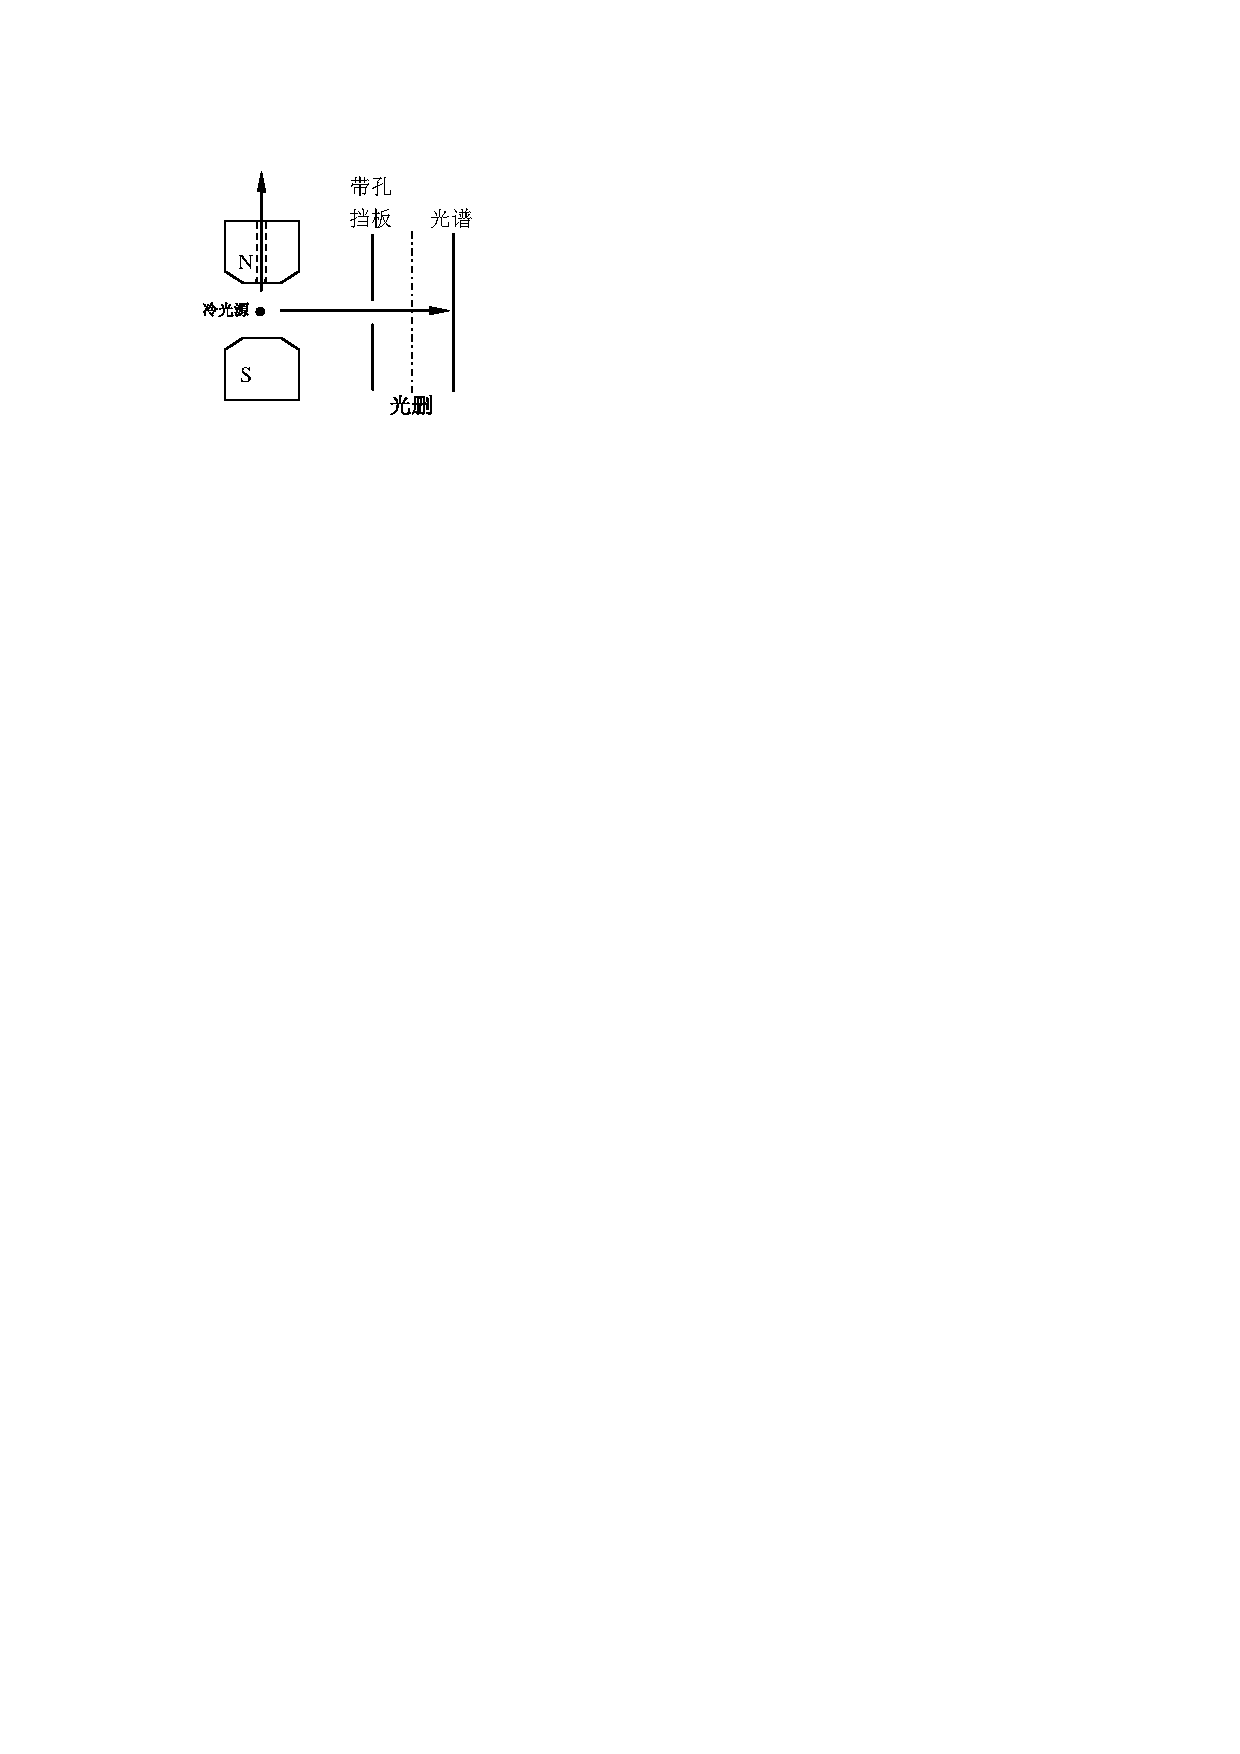
\includegraphics[width=0.7\textwidth]{fig07.pdf}
\caption{\label{fig08}塞曼效应实验装置}
\end{minipage}%
\begin{minipage}[b]{0.48\textwidth}
\centering
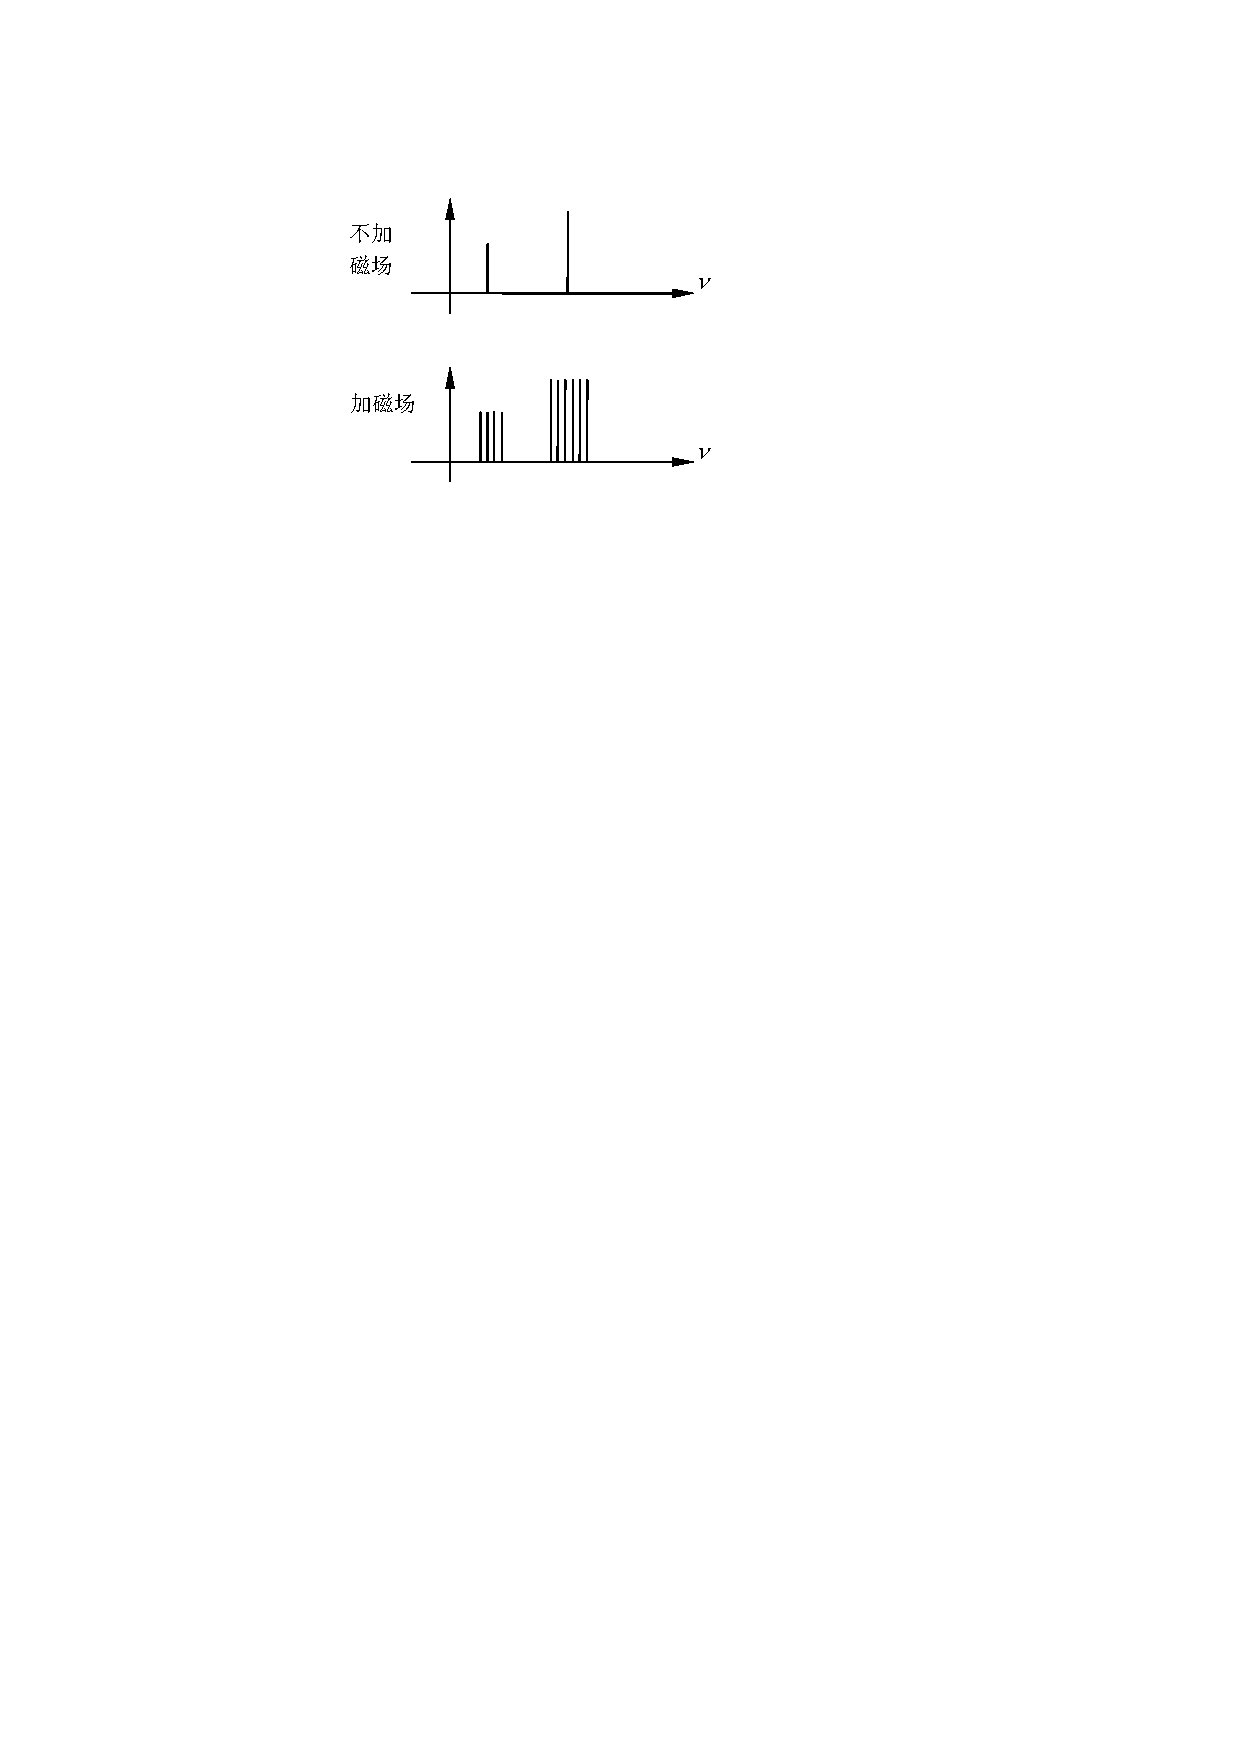
\includegraphics[width=0.7\textwidth]{fig14.pdf}
\caption{\label{fig09}塞曼效应的结果}
\end{minipage}
\end{figure}
\textbf{注意}: 塞曼效应的光谱为偏振光谱, 谱线对称分裂. 

\subsection{斯塔克(Stark)效应}
斯坦克效应是原子发出的谱线在电场作用下产生分裂的一种现象. 
\begin{figure}[!htb]
\begin{minipage}[b]{0.48\textwidth}
\centering
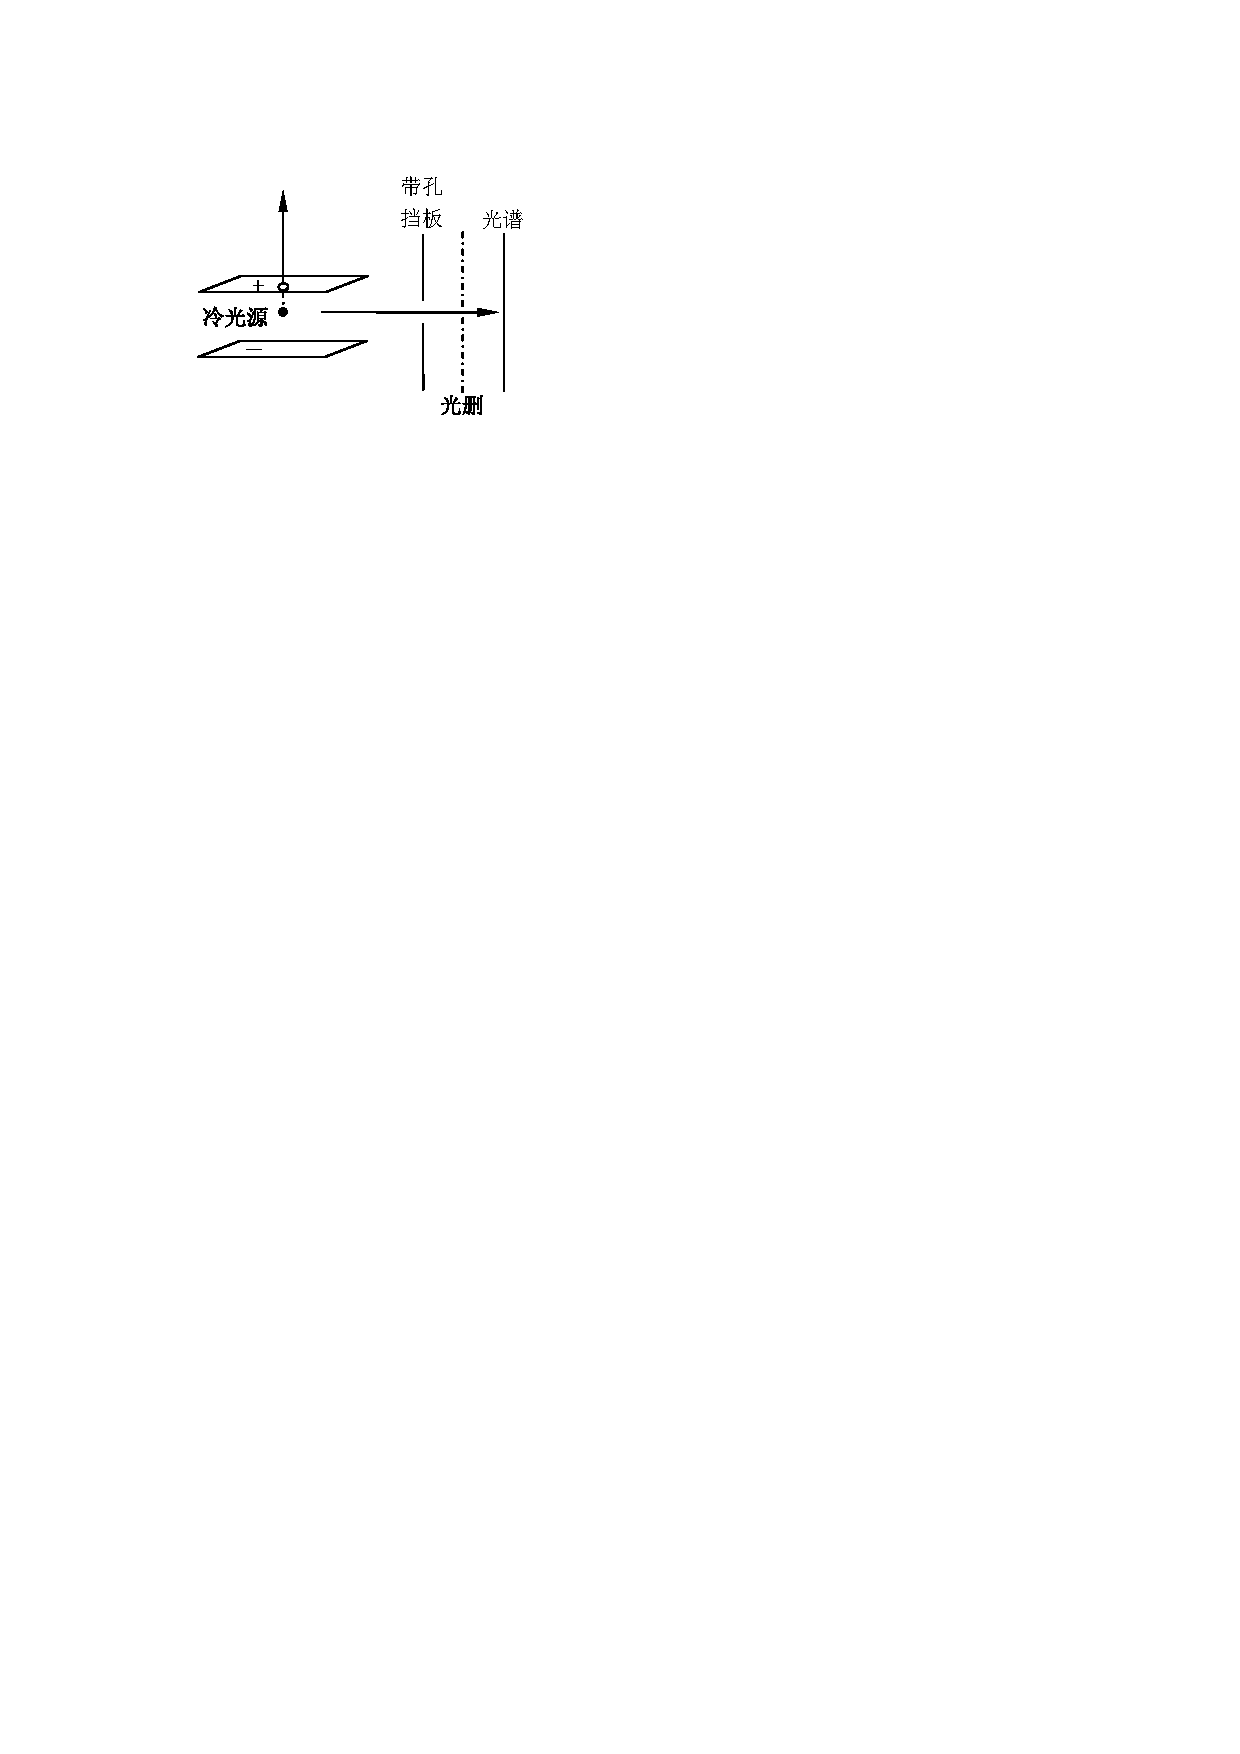
\includegraphics[width=0.7\textwidth]{fig08.pdf}
\caption{\label{fig08}斯坦克效应实验装置}
\end{minipage}%
\begin{minipage}[b]{0.48\textwidth}
\centering
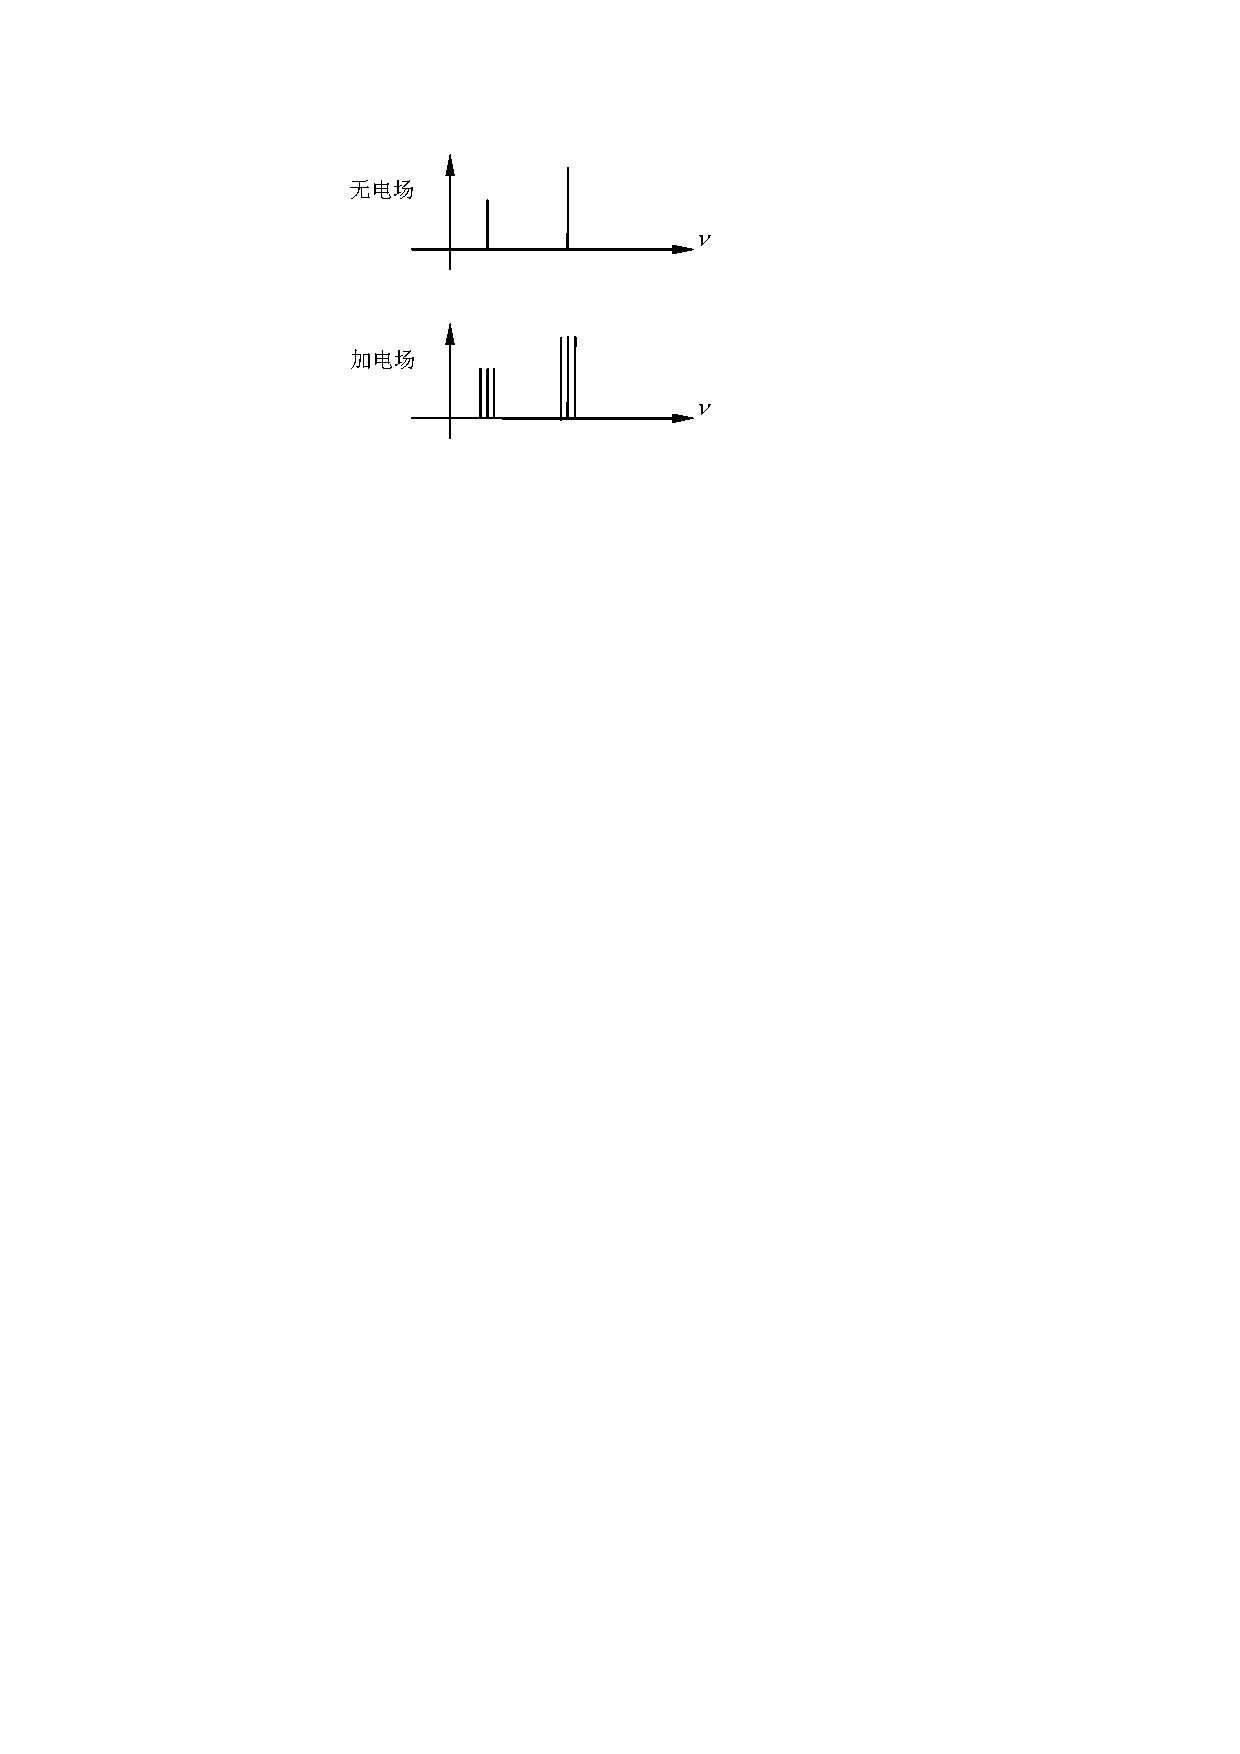
\includegraphics[width=0.7\textwidth]{fig09.pdf}
\caption{\label{fig09}斯坦克效应的结果}
\end{minipage}
\end{figure}
\textbf{结果}: 加电场后, 谱线由一条分裂成三条(如图\ref{fig09}), 并且对于氢原子有$\Delta\mu\propto E$(一级斯坦克效应)
